\documentclass[t, aspectratio=169]{beamer}
\usepackage{amsmath,amsfonts,amsthm,amstext,amssymb, xcolor, tikz, pgf, mathrsfs, polynom, pifont, tabto}

% ----------------------------------------------------------
% Theme Setup

% Use Metropolis Theme
\usetheme[numbering=fraction]{metropolis}
\setbeamertemplate{blocks}[rounded][shadow=false]
\makeatletter
\setlength{\metropolis@titleseparator@linewidth}{1pt}
\makeatother

% Define Colors
\definecolor{chargerblue}{HTML}{002764}
\definecolor{chargerred}{HTML}{e02034}
\definecolor{bggray}{HTML}{d0d3d4}

% Set Colors
\setbeamercolor{title}{fg=chargerblue}
\setbeamercolor{background canvas}{bg=white}
\setbeamercolor{title separator}{fg=chargerred}
\setbeamercolor{structure}{fg=chargerblue}
\setbeamercolor{frametitle}{fg=white, bg=chargerblue}
\setbeamercolor*{normal text}{fg=chargerblue}
\setbeamercolor*{block body}{bg=bggray}
\setbeamercolor*{block title}{bg=chargerblue, fg=white}
% ----------------------------------------------------------

% ----------------------------------------------------------
% Custom Definitions, Commands, Environments, etc.

% Sets of numbers
\def\R{\mathbb{R}} % The reals
\def\N{\mathbb{N}} % The naturals
\def\Z{\mathbb{Z}} % The integers
\def\Q{\mathbb{Q}} % The rationals

% Blank space
\newcommand{\blank}[1]{\underline{\hspace{#1}}} % Blank space

% Change font colors
\newcommand{\cyan}[1]{{\color{cyan}{#1}}} % Changes font to cyan
\newcommand{\red}[1]{{\color{red}{#1}}} % Changes font to red
\newcommand{\magenta}[1]{{\color{magenta}{#1}}} % Changes font to magenta
\newcommand{\orange}[1]{{\color{orange}{#1}}} % Changes font to orange
\newcommand{\yellow}[1]{{\color{yellow}{#1}}} % Changes font to yellow
\newcommand{\violet}[1]{{\color{violet}{#1}}} % Changes font to violet
\newcommand{\green}[1]{{\color{green}{#1}}} % Changes font to green
\newcommand{\blue}[1]{{\color{blue}{#1}}} % Changes font to blue
\newcommand{\white}[1]{{\color{white}{#1}}} % Changes font to white

% Fitted inclusion symbols
\newcommand{\fp}[1]{\left({#1}\right)} % Fitted parentheses around content
\newcommand{\fb}[1]{\left[{#1}\right]} % Fitted brackets
\newcommand{\lhoi}[1]{\left({#1}\right]} % Left half-open interval
\newcommand{\rhoi}[1]{\left[{#1}\right)} % Right half-open interval
\newcommand{\set}[1]{\left\{{#1}\right\}} % Fitted braces (useful for sets)
\newcommand{\av}[1]{\left|{#1}\right|} % Fitted absolute value bars

% Augmented Matrix Environment
\newenvironment{amatrix}[1]{%
	\left[\begin{array}{@{}*{#1}{c}|c@{}}
	}{%
	\end{array}\right]
}

% Miscellaneous
\def\then{\Rightarrow}
\def\to{\rightarrow}
\def\d{^{\circ}}
\newcommand{\?}{\stackrel{?}{=}}
\newcommand{\cmark}{\text{ \ding{51}}}
\newcommand{\xmark}{\text{ \ding{55}}}

% Coordinate Plane (Four-Quadrant)
\def\coordplane {
	\begin{tikzpicture}        \draw[step=0.25cm,black,very thin,opacity=0.25] (-2.5cm, -2.5cm) grid (2.5cm, 2.5cm);
		\draw[<->,thick,black] (-2.5cm, 0) -- (2.5cm, 0) node[anchor=north west,pos=0.94,font=\scriptsize]{$x$};
		\draw[<->,thick,black] (0,-2.5cm) -- (0, 2.5cm) node[anchor=south east,font=\scriptsize,pos=0.94]{$y$};
	\end{tikzpicture}
}

% Coordinate Plane (One-Quadrant)
\def\onequad {
	\begin{tikzpicture}
		\draw[step=0.25cm, black, very thin, opacity=0.25] (0,0) grid (7.5cm,5cm);
		\draw[->, thick, black] (0,0) -- (7.5cm, 0) node[anchor=north west,font=\scriptsize,pos=0.94]{$x$};
		\draw[->, black, thick] (0,0) -- (0,5cm) node[anchor=south east,font=\scriptsize,pos=0.94]{$y$};
	\end{tikzpicture}
}
% ----------------------------------------------------------

% ----------------------------------------------------------
% Presentation Information
\title[3-4]{Exploratory Data Analysis}
\subtitle{Section 3-4}
\author{Jacob Ayers}
\institute{Lesson \#8}
\date{MAT 110}
% ----------------------------------------------------------

\begin{document}
	
	% Slide 1 (Title Slide)
	\begin{frame}
		\titlepage
	\end{frame}
	
	% Slide 2 (Objectives)
	\begin{frame}{Objectives}
		\begin{itemize}
			\item Find the five-number-summary of a data set
			\item Construct boxplots
		\end{itemize}
	\end{frame}

	\begin{frame}{Exploratory Data Analysis}
		Purpose of analysis: confirm various conjectures about data \pause
		
		In exploratory data analysis (EDA), we organize data using stem-and-leaf plots. \begin{itemize}
			\item Measure of central tendency: median
			\item Measure of variation: IQR
			\item Graphical representation: Boxplot (aka box-and-whisker plot)
		\end{itemize} \pause
	
		Purpose of EDA: find out what information can be discovered about the data (e.g. center and spread)
	\end{frame}

	\begin{frame}{The Five-Number Summary}
		The \textit{five-number summary} of a data set includes the following values: \begin{itemize}
			\item The lowest value (minimum) \pause
			\item $Q_1$ \pause
			\item The median \pause
			\item $Q_3$ \pause
			\item The highest value (maximum)
		\end{itemize} \pause
	
		I'll be demonstrating finding the five-number summary using a calculator, but it can also be done by hand using methods we've seen in previous videos.
	\end{frame}

	\begin{frame}{The Five-Number Summary}
		Identify the five-number summary and find the interquartile range for the data.
		
		$362, 589, 437, 316, 192, 188$ \pause
		
		Using a graphing calculator: \\
		Min = 188 \\
		$Q_1$ = 192 \\
		Median = 339 \\
		$Q_3$ = 437 \\
		Max = 589 \\
		IQR = $437 - 192 = 245$
	\end{frame}

	\begin{frame}{Boxplots}
		Once we have the five-number summary, we can draw a boxplot. \pause
		
		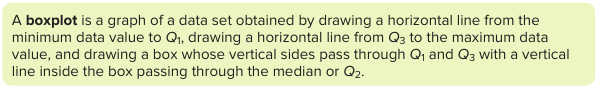
\includegraphics[width=5in]{box-def.png} \pause
		
		We don't have a great method of constructing a boxplot on a calculator or in Sheets, so we'll have to draw them by hand.
	\end{frame}

	\begin{frame}{Boxplots}
		The number of meteorites found in 10 states of the United States is 89, 47, 164, 296, 30, 215, 138, 78, 48, 39. Construct a boxplot for the data. \pause
		
		First, find the five-number summary (30, 47, 83.5, 164, 296). \pause
		
		Now, we can draw the boxplot.
	\end{frame}

	\begin{frame}{Boxplots}
		Construct a boxplot for the data below.
		
		79, 82, 77, 84, 80, 89, 60, 79, 91, 93, 88
		
		First, find the find-number summary (60, 79, 82, 89, 93). \pause
		
		Now, we can draw the boxplot.
	\end{frame}

	\begin{frame}{Next Steps}
		\begin{itemize}
			\item Prepare for Midterm 1
			\item Take Midterm 1
			\item Begin Module \#6 \begin{itemize}
				\item Read 4-1
				\item Watch Video Lesson \#9
			\end{itemize}
		\end{itemize}
	
		\vfill
		
		Thanks for watching!
	\end{frame}
	
\end{document}